\documentclass{standalone}
\usepackage{tikz,pgfplots}
\pgfplotsset{compat=newest}
\begin{document}

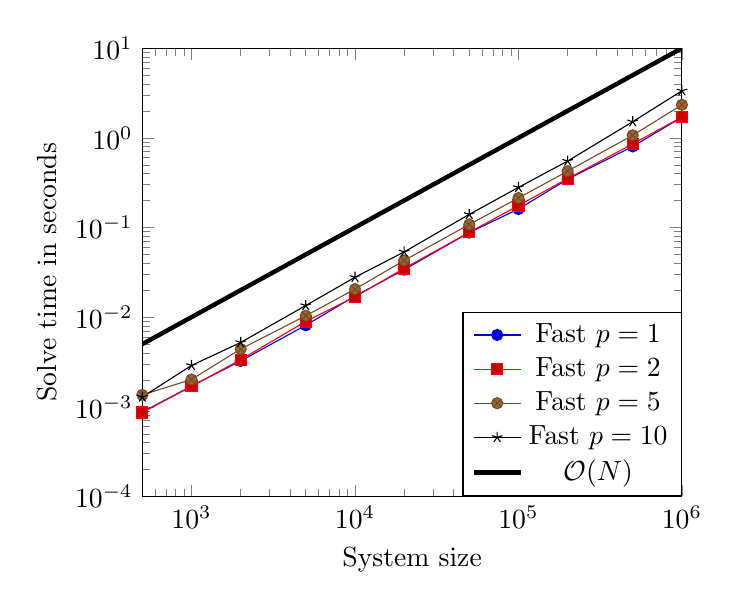
\begin{tikzpicture}
\begin{loglogaxis}[
	xlabel={System size},
	ylabel={Solve time in seconds},
	xmin=500, xmax=1000000,
	ymin=1e-4, ymax=1e1,
	legend style={
  		at={(1.0,0.0)},
		anchor=south east},
]
%Fast p=1
\addplot
coordinates{
(500, 0.000874) (1000, 0.001705) (2000, 0.003251) (5000, 0.008114) (10000, 0.017188) (20000, 0.033885) (50000, 0.087764) (100000, 0.1606) (200000, 0.345631) (500000, 0.801305) (1000000, 1.70053) 
};
\addlegendentry{Fast $p=1$}
%Fast p=2
\addplot
coordinates{
(500, 0.000864) (1000, 0.001689) (2000, 0.003353) (5000, 0.008956) (10000, 0.01686) (20000, 0.034964) (50000, 0.088298) (100000, 0.175811) (200000, 0.350503) (500000, 0.855516) (1000000, 1.70446) 
};
\addlegendentry{Fast $p=2$}
%Fast p=5
\addplot
coordinates{
(500, 0.001357) (1000, 0.002017) (2000, 0.004414) (5000, 0.010366) (10000, 0.020525) (20000, 0.042892) (50000, 0.108075) (100000, 0.213189) (200000, 0.425323) (500000, 1.06771) (1000000, 2.33446) 
};
\addlegendentry{Fast $p=5$}
%Fast p=10
\addplot
coordinates{
(500, 0.001287) (1000, 0.002892) (2000, 0.005222) (5000, 0.013472) (10000, 0.027853) (20000, 0.053413) (50000, 0.139973) (100000, 0.279942) (200000, 0.550983) (500000, 1.51185) (1000000, 3.3476) 
};
\addlegendentry{Fast $p=10$}
%O(N) scaling
\addplot[ultra thick, no marks]
coordinates{
(500, 0.005) (1000000, 10)
};
\addlegendentry{$\mathcal{O}(N)$}
% %O(N^2) scaling
% \addplot
% coordinates{
% (500, 0.01) (10000, 4)
% };
% \addlegendentry{$\mathcal{O}(N^2)$}
% %Usual
% \addplot
% coordinates{
% (500, 0.000237) (1000, 0.000854) (2000, 0.002744) (5000, 0.013979) (10000, 0.061031)
% };
% \addlegendentry{Usual}
\end{loglogaxis}
\end{tikzpicture}
\end{document}